\documentclass{article}
\setlength{\paperheight}{45cm}
\setlength{\paperwidth}{32cm}
\setlength{\headheight}{0pt}
\setlength{\headsep}{0pt}
\setlength{\footskip}{0pt}
\setlength{\textwidth}{\paperwidth}
\addtolength{\textwidth}{-5cm}
\setlength{\oddsidemargin}{0pt}
\setlength{\evensidemargin}{\oddsidemargin}
\setlength{\textheight}{\paperheight}
\setlength{\topmargin}{0pt}
\addtolength{\topmargin}{0pt}
\setlength{\parindent}{0pt}

\usepackage{pgfpages}
\pgfpagesuselayout{resize to}[a4paper]

\usepackage{tikz}
\usetikzlibrary{arrows,decorations.pathmorphing,backgrounds,positioning,fit,shapes.geometric,shapes.symbols,shapes.multipart,topaths}
\usepackage{pgf-umlsd}

\large

\tikzstyle{box}=[rectangle,outer sep=2mm,inner sep=2mm,draw,rounded corners=0.5mm,text centered,line width=0.2mm]
\tikzstyle{class}=[box,draw=blue,text=white,fill=cyan]
\tikzstyle{role}=[box,draw=gray!70,text=black,fill=gray!80]
\tikzstyle{package}=[box,draw=gray!70,text=black,fill=gray!80]
\tikzstyle{class plus}=[box,rectangle split,rectangle split parts=2,rectangle split part align={center,left},draw=blue,text=white,rectangle split part fill={cyan,gray!60}]

\tikzstyle{isa}=[-open triangle 60,thin]
\tikzstyle{does}=[-open triangle 60,thin,dashed]
\tikzstyle{uses}=[-stealth',thick]
\tikzstyle{has a}=[diamond-,thin]
\tikzstyle{shared has a}=[open diamond-,thin]
\tikzstyle{magic arrow}=[->,double equal sign distance,double,thick]

\begin{document}

\section{Key}

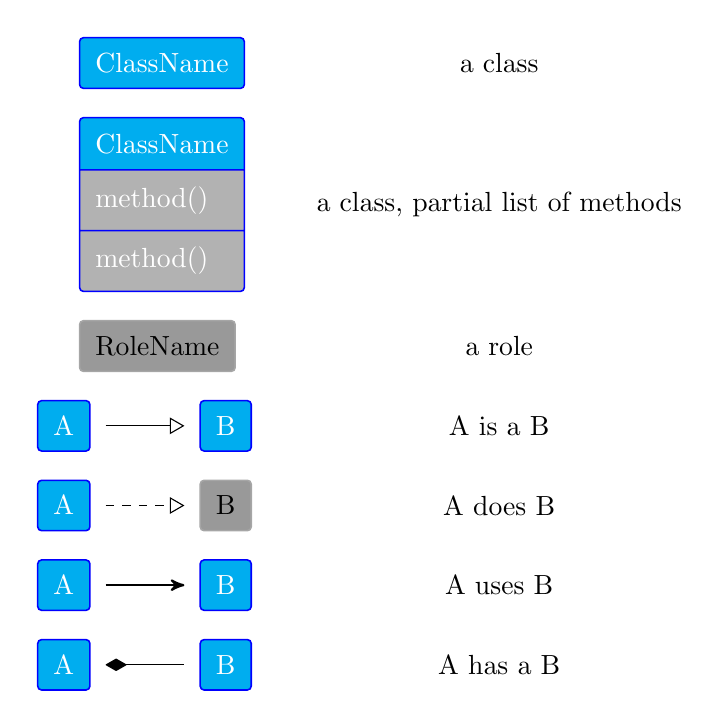
\begin{tikzpicture}

\matrix[row sep=1em,column sep=2em] {
  \node [class,anchor=west] {ClassName} ; & \node {a class} ; \\
  \node [class plus,rectangle split parts=3,anchor=west] {ClassName \nodepart{two} method() \nodepart{three} method() } ; & \node {a class, partial list of methods}; \\
  \node [role,anchor=west] {RoleName} ; & \node {a role} ; \\
  \node (a) [class] {A} ; \node (b) [class,right=of a] {B} ; \draw [isa] (a) -- (b) ; & \node {A is a B} ; \\
  \node (a) [class] {A} ; \node (b) [role,right=of a] {B} ; \draw [does] (a) -- (b) ; & \node {A does B} ; \\
  \node (a) [class] {A} ; \node (b) [class,right=of a] {B} ; \draw [uses] (a) -- (b) ; & \node {A uses B} ; \\
  \node (a) [class] {A} ; \node (b) [class,right=of a] {B} ; \draw [has a] (a) -- (b) ; & \node {A has a B} ; \\
};

\end{tikzpicture}

\section{Sending messages}

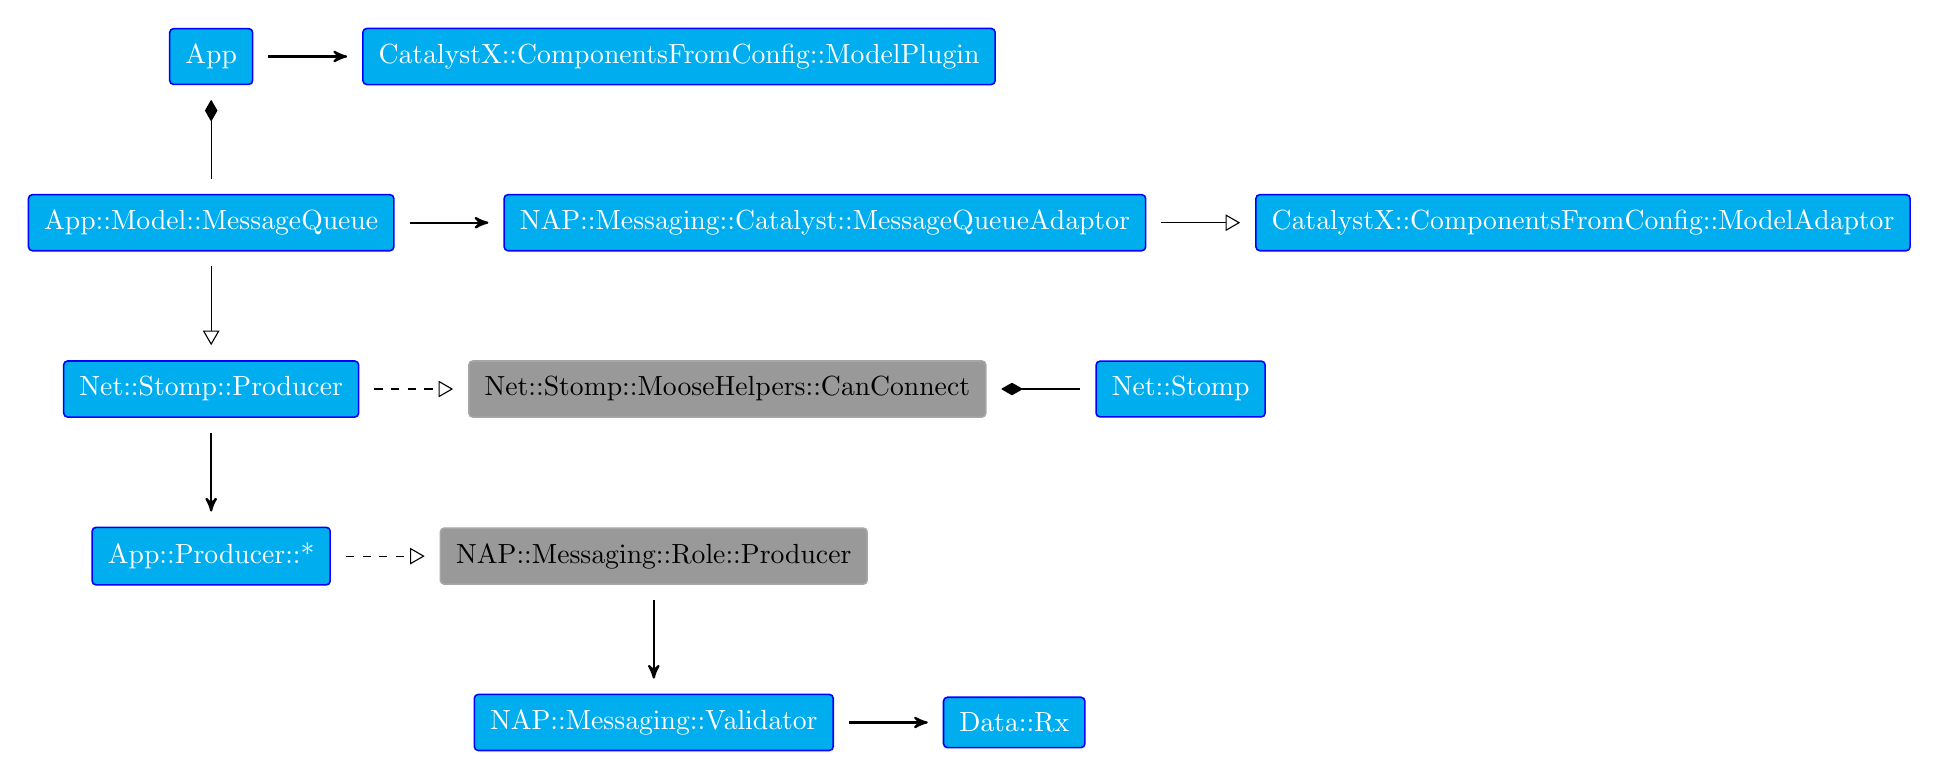
\begin{tikzpicture}

\node (app) [class] {App} ;
\node (mq) [class,below=of app] {App::Model::MessageQueue} ;
\node (cfc-mp) [class,right=of app] {CatalystX::ComponentsFromConfig::ModelPlugin} ;
\node (mqa) [class,right=of mq] {NAP::Messaging::Catalyst::MessageQueueAdaptor} ;
\node (cfc-ma) [class,right=of mqa] {CatalystX::ComponentsFromConfig::ModelAdaptor} ;

\draw [uses] (app) -- (cfc-mp) ;
\draw [has a] (app) -- (mq) ;
\draw [uses] (mq) -- (mqa) ;
\draw [isa] (mqa) -- (cfc-ma) ;

\node (nsprod) [class,below=of mq] {Net::Stomp::Producer} ;
\node (nsmhcc) [role,right=of nsprod] {Net::Stomp::MooseHelpers::CanConnect} ;
\node (ns) [class,right=of nsmhcc] {Net::Stomp} ;

\draw [isa] (mq) -- (nsprod) ;
\draw [does] (nsprod) -- (nsmhcc) ;
\draw [has a] (nsmhcc) -- (ns) ;

\node (prod) [class,below=of nsprod] {App::Producer::*} ;
\node (prodrole) [role,right=of prod] {NAP::Messaging::Role::Producer} ;
\node (val) [class,below=of prodrole] {NAP::Messaging::Validator} ;
\node (rx) [class,right=of val] {Data::Rx} ;

\draw [uses] (nsprod) -- (prod) ;
\draw [does] (prod) -- (prodrole) ;
\draw [uses] (prodrole) -- (val) ;
\draw [uses] (val) -- (rx) ;

\end{tikzpicture}

\section{Consumer application}

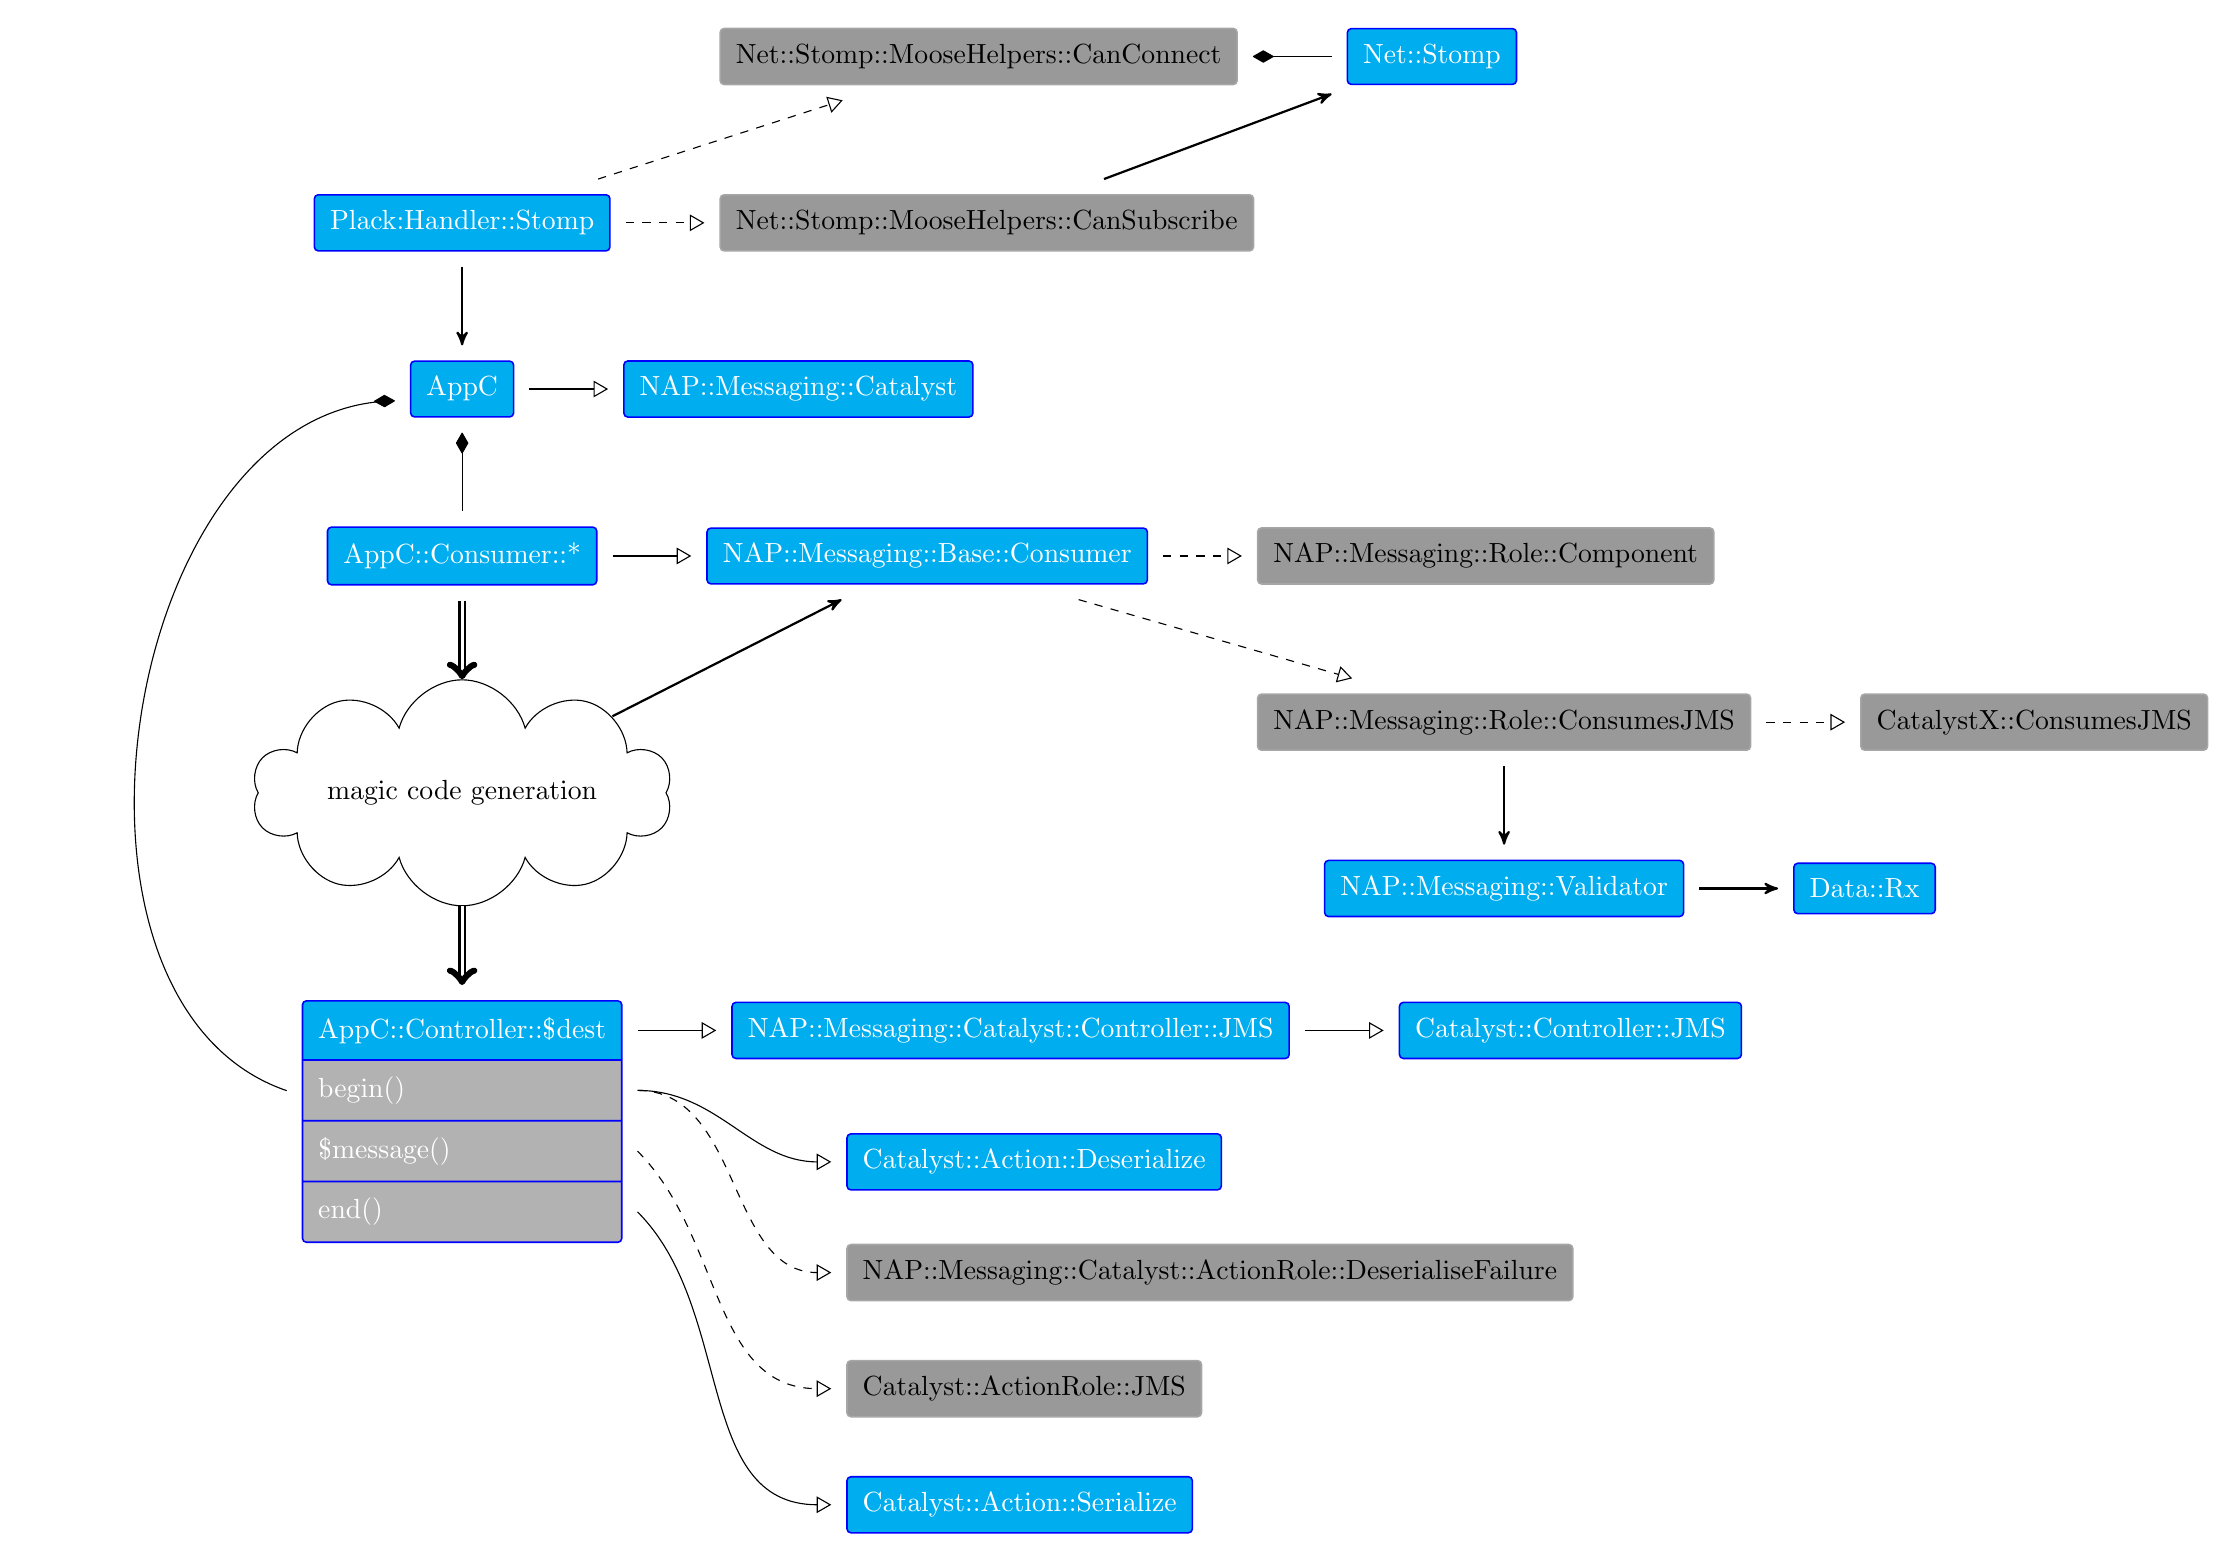
\begin{tikzpicture}

\node (appc) [class] {AppC} ;
\node (cat) [class,right=of appc] {NAP::Messaging::Catalyst} ;

\node (phs) [class,above=of appc] {Plack:Handler::Stomp };
\node (nsmhcc) [role,above right=of phs] {Net::Stomp::MooseHelpers::CanConnect} ;
\node (nsmhcs) [role,right=of phs] {Net::Stomp::MooseHelpers::CanSubscribe} ;
\node (ns) [class,right=of nsmhcc] {Net::Stomp} ;

\draw [isa] (appc) -- (cat) ;
\draw [uses] (phs) -- (appc) ;
\draw [does] (phs) -- (nsmhcc) ;
\draw [does] (phs) -- (nsmhcs) ;
\draw [has a] (nsmhcc) -- (ns) ;
\draw [uses] (nsmhcs) -- (ns) ;

\node (cons) [class,below=of appc] {AppC::Consumer::*} ;
\node (bcons) [class,right=of cons] {NAP::Messaging::Base::Consumer} ;
\node (comp) [role,right=of bcons] {NAP::Messaging::Role::Component} ;
\node (jms) [role,below right=of bcons] {NAP::Messaging::Role::ConsumesJMS} ;
\node (bjms) [role,right=of jms] {CatalystX::ConsumesJMS} ;
\node (val) [class,below=of jms] {NAP::Messaging::Validator} ;
\node (rx) [class,right=of val] {Data::Rx} ;

\draw [has a] (appc) -- (cons) ;
\draw [isa] (cons) -- (bcons) ;
\draw [does] (bcons) -- (comp) ;
\draw [does] (bcons) -- (jms) ;
\draw [does] (jms) -- (bjms) ;
\draw [uses] (jms) -- (val) ;
\draw [uses] (val) -- (rx) ;

\node (magic-codegen) [cloud,draw,aspect=3,below=of cons] {magic code generation} ;

\node (cc) [class plus,rectangle split parts=4,below=of magic-codegen] {
   AppC::Controller::\$dest
   \nodepart{two} begin()
   \nodepart{three} \$message()
   \nodepart{four} end()
} ;
\node (nmjms) [class,right=of cc.one east] {NAP::Messaging::Catalyst::Controller::JMS} ;
\node (ccjms) [class,right=of nmjms] {Catalyst::Controller::JMS} ;
\node (cads) [class,below right=1em and 7em of cc.two east] {Catalyst::Action::Deserialize} ;
\node (nmfail) [role,below right=5em and 7em of cc.two east] {NAP::Messaging::Catalyst::ActionRole::DeserialiseFailure} ;
\node (carjms) [role,below right=7em and 7em of cc.three east] {Catalyst::ActionRole::JMS} ;
\node (cas) [class,below right=9em and 7em of cc.four east] {Catalyst::Action::Serialize} ;

\draw [has a] (appc) to [bend right=80] (cc) ;
\draw [isa] (cc.one east) -- (nmjms) ;
\draw [isa] (nmjms) -- (ccjms) ;
\draw [isa] (cc.two east) to[out=0,in=180] (cads) ;
\draw [does] (cc.two east) to[out=0,in=180] (nmfail) ;
\draw [does] (cc.three east) to[out=-45,in=180] (carjms) ;
\draw [isa] (cc.four east) to[out=-45,in=180] (cas) ;

\draw [magic arrow] (cons) -- (magic-codegen) ;
\draw [magic arrow] (magic-codegen) -- (cc) ;
\draw [uses] (magic-codegen) -- (bcons) ;

\end{tikzpicture}

\end{document}
